\chapter{Data Manipulation and Its Representation}\label{introduction-to-python---lesson-5}

\begin{Exercise}
Using \texttt{pandas} import data stored in \href{https://drive.google.com/file/d/1Uu9lQorvzM-1xwRKPNszaSqlCYAiY-gr/view?usp=sharing}{\texttt{stock\_market.xlsx}} (click on the name to see and download it). With the resulting dataframe determine:
\Question remove duplicates and missing data (how many rows are left ?)
\Question stocks with positive variation;
\Question the first five stocks with the lowest price.
\end{Exercise}
\clearpage
\begin{Answer}
  \Question
First load the excel file into a dataframe and look at data structure.

\begin{codebox}[size=fbox, boxrule=1pt, colback=cellbackground, colframe=cellborder]
\begin{Verbatim}[commandchars=\\\{\}]
\PY{k+kn}{import} \PY{n+nn}{pandas} \PY{k}{as} \PY{n+nn}{pd}

\PY{n}{df} \PY{o}{=} \PY{n}{pd}\PY{o}{.}\PY{n}{read\PYZus{}excel}\PY{p}{(}\PY{l+s+s2}{\PYZdq{}}\PY{l+s+s2}{stock\PYZus{}market.xlsx}\PY{l+s+s2}{\PYZdq{}}\PY{p}{)}

\PY{n+nb}{print} \PY{p}{(}\PY{n+nb}{len}\PY{p}{(}\PY{n}{df}\PY{p}{)}\PY{p}{)}
\PY{n}{df}\PY{o}{.}\PY{n}{head}\PY{p}{(}\PY{p}{)}

51

  Symbol                      Name   Price  Change  Change\%  Volume (M)  \textbackslash{}
0     GE  General Electric Company    6.07   -0.19  -0.0304     142.732
1    NOK         Nokia Corporation    4.78    0.33   0.0742     117.960
2      F        Ford Motor Company    6.61   -0.13  -0.0193     115.394
3   PINS           Pinterest, Inc.   34.29    9.10   0.3613     111.864
4   AAPL                Apple Inc.  425.04   40.28   0.1047      93.574

   Avg Volume (M)  Market Cap (B)
0         102.268          53.132
1          31.296          27.083
2          87.719          26.288
3          15.550          20.110
4          35.035        1821.000
\end{Verbatim}
\end{codebox}
        
As usual if we are not sure that our data is \emph{clean} we should check for duplicates and NaN and take care of them. The \texttt{duplicated} method returns the status of each row (duplicate or not, True or False). If we would like just to see the duplicated entries we could combine the \texttt{duplicated} method with the selection syntax like this:

\begin{codebox}[size=fbox, boxrule=1pt, colback=cellbackground, colframe=cellborder]
\begin{Verbatim}[commandchars=\\\{\}]
\PY{n}{df}\PY{p}{[}\PY{n}{df}\PY{o}{.}\PY{n}{duplicated}\PY{p}{(}\PY{p}{)} \PY{o}{==} \PY{k+kc}{True}\PY{p}{]}

   Symbol         Name  Price  Change  Change\%  Volume (M)  Avg Volume (M)  \textbackslash{}
40    RUN  Sunrun Inc.  36.69    0.02   0.0005      20.113           3.604

    Market Cap (B)
40           4.489
\end{Verbatim}
\end{codebox}
        
So it looks like we have just one duplicate and we can remove it:

\begin{codebox}[size=fbox, boxrule=1pt, colback=cellbackground, colframe=cellborder]
\begin{Verbatim}[commandchars=\\\{\}]
\PY{n+nb}{print} \PY{p}{(}\PY{l+s+s2}{\PYZdq{}}\PY{l+s+s2}{Before duplicates removal: }\PY{l+s+si}{\PYZob{}\PYZcb{}}\PY{l+s+s2}{\PYZdq{}}\PY{o}{.}\PY{n}{format}\PY{p}{(}\PY{n+nb}{len}\PY{p}{(}\PY{n}{df}\PY{p}{)}\PY{p}{)}\PY{p}{)}
\PY{n}{df} \PY{o}{=} \PY{n}{df}\PY{o}{.}\PY{n}{drop\PYZus{}duplicates}\PY{p}{(}\PY{p}{)}
\PY{n+nb}{print} \PY{p}{(}\PY{l+s+s2}{\PYZdq{}}\PY{l+s+s2}{After duplicates removal: }\PY{l+s+si}{\PYZob{}\PYZcb{}}\PY{l+s+s2}{\PYZdq{}}\PY{o}{.}\PY{n}{format}\PY{p}{(}\PY{n+nb}{len}\PY{p}{(}\PY{n}{df}\PY{p}{)}\PY{p}{)}\PY{p}{)}

Before duplicates removal: 50
After duplicates removal: 50
\end{Verbatim}
\end{codebox}

Then we need to take care of the NaN, again if we want to check the rows with NaN we can select (here the syntax is a little bit more complicated since we need to use \texttt{any} to look for Nan in every column):

\begin{codebox}[size=fbox, boxrule=1pt, colback=cellbackground, colframe=cellborder]
\begin{Verbatim}[commandchars=\\\{\}]
\PY{n}{df}\PY{p}{[}\PY{n}{df}\PY{o}{.}\PY{n}{isna}\PY{p}{(}\PY{p}{)}\PY{o}{.}\PY{n}{any}\PY{p}{(}\PY{n}{axis}\PY{o}{=}\PY{l+m+mi}{1}\PY{p}{)}\PY{p}{]}

   Symbol                                 Name  Price  Change  Change\%  \textbackslash{}
23   NCLH  Norwegian Cruise Line Holdings Ltd.  13.64   -0.53  -0.0374
47    NBL                   Noble Energy, Inc.    NaN   -0.23  -0.0225

    Volume (M)  Avg Volume (M)  Market Cap (B)
23      28.402          64.895             NaN
47      18.462          13.535           4.795
\end{Verbatim}
\end{codebox}
        
Since we don't want to artificially modify our sample we just drop rows with NaN:

\begin{codebox}[size=fbox, boxrule=1pt, colback=cellbackground, colframe=cellborder]
\begin{Verbatim}[commandchars=\\\{\}]
\PY{n+nb}{print} \PY{p}{(}\PY{l+s+s2}{\PYZdq{}}\PY{l+s+s2}{Before NaN removal: }\PY{l+s+si}{\PYZob{}\PYZcb{}}\PY{l+s+s2}{\PYZdq{}}\PY{o}{.}\PY{n}{format}\PY{p}{(}\PY{n+nb}{len}\PY{p}{(}\PY{n}{df}\PY{p}{)}\PY{p}{)}\PY{p}{)}
\PY{n}{df} \PY{o}{=} \PY{n}{df}\PY{o}{.}\PY{n}{dropna}\PY{p}{(}\PY{p}{)}
\PY{n+nb}{print} \PY{p}{(}\PY{l+s+s2}{\PYZdq{}}\PY{l+s+s2}{After NaN removal: }\PY{l+s+si}{\PYZob{}\PYZcb{}}\PY{l+s+s2}{\PYZdq{}}\PY{o}{.}\PY{n}{format}\PY{p}{(}\PY{n+nb}{len}\PY{p}{(}\PY{n}{df}\PY{p}{)}\PY{p}{)}\PY{p}{)}

Before NaN removal: 51
After NaN removal: 49
\end{Verbatim}
\end{codebox}

\Question
The second point asks to determine the companies with a daily positive variation. Clearly we have to apply to the dataframe a selection on the ``Change'' (or ``Change\%'') column requiring positive values.

\begin{codebox}[size=fbox, boxrule=1pt, colback=cellbackground, colframe=cellborder]
\begin{Verbatim}[commandchars=\\\{\}]
\PY{n}{pos\PYZus{}var} \PY{o}{=} \PY{n}{df}\PY{p}{[}\PY{n}{df}\PY{o}{.}\PY{n}{loc}\PY{p}{[}\PY{p}{:}\PY{p}{,} \PY{l+s+s2}{\PYZdq{}}\PY{l+s+s2}{Change}\PY{l+s+s2}{\PYZdq{}}\PY{p}{]} \PY{o}{\PYZgt{}} \PY{l+m+mi}{0}\PY{p}{]}

\PY{n+nb}{print} \PY{p}{(}\PY{n+nb}{len}\PY{p}{(}\PY{n}{pos\PYZus{}var}\PY{p}{)}\PY{p}{)}
\PY{n}{pos\PYZus{}var}\PY{o}{.}\PY{n}{head}\PY{p}{(}\PY{p}{)} \PY{c+c1}{\PYZsh{} just printing the first 5 rows}

16

  Symbol                         Name   Price  Change  Change\%  Volume (M)  \textbackslash{}
1    NOK            Nokia Corporation    4.78    0.33   0.0742     117.960
3   PINS              Pinterest, Inc.   34.29    9.10   0.3613     111.864
4   AAPL                   Apple Inc.  425.04   40.28   0.1047      93.574
6    BAC  Bank of America Corporation   24.88    0.04   0.0016      62.039
8     FB               Facebook, Inc.  253.67   19.17   0.0817      53.030

   Avg Volume (M)  Market Cap (B)
1          31.296          27.083
3          15.550          20.110
4          35.035        1821.000
6          72.793         215.562
8          24.521         723.726
\end{Verbatim}
\end{codebox}
        
So in origin we had 48 stocks and just 16 have a positive variation of its price.

\Question
The last question requires to print the first 5 stocks with the lowest prices. In this case it is enough to sort by price the dataframe (ascending) and then just select the first 5 entries.

\begin{codebox}[size=fbox, boxrule=1pt, colback=cellbackground, colframe=cellborder]
\begin{Verbatim}[commandchars=\\\{\}]
\PY{n}{highest\PYZus{}price} \PY{o}{=} \PY{n}{df}\PY{o}{.}\PY{n}{sort\PYZus{}values}\PY{p}{(}\PY{n}{by}\PY{o}{=}\PY{p}{[}\PY{l+s+s1}{\PYZsq{}}\PY{l+s+s1}{Price}\PY{l+s+s1}{\PYZsq{}}\PY{p}{]}\PY{p}{,} \PY{n}{ascending}\PY{o}{=}\PY{k+kc}{True}\PY{p}{)}\PY{p}{[}\PY{p}{:}\PY{l+m+mi}{5}\PY{p}{]}

\PY{n}{highest\PYZus{}price}

   Symbol                      Name  Price  Change  Change\%  Volume (M)  \textbackslash{}
25   ABEV               Ambev S. A.   2.68   -0.16  -0.0563      26.136
32    BBD      Banco Bradesco S. A.   4.22   -0.32  -0.0705      22.129
1     NOK         Nokia Corporation   4.78    0.33   0.0742     117.960
15    OPK         OPKO Health, Inc.   5.15   -0.76  -0.1286      35.762
33    MRO  Marathon Oil Corporation   5.49   -0.02  -0.0036      21.249

    Avg Volume (M)  Market Cap (B)
25          36.654          41.999
32          22.046          36.739
1           31.296          27.083
15          17.792           3.450
33          34.098           4.339
\end{Verbatim}
\end{codebox}
\end{Answer}

\begin{Exercise}
Given the following discount factors plot the resulting discount curve,
possibly adding axis labels and legend.

\begin{Shaded}
\begin{Highlighting}[]
\NormalTok{dfs }\OperatorTok{=}\NormalTok{ [}\FloatTok{1.0}\NormalTok{, }\FloatTok{1.0014907894567657}\NormalTok{, }\FloatTok{1.0031038833235129}\NormalTok{, }\FloatTok{1.0047764800189012}\NormalTok{,}
       \FloatTok{1.0065986105304596}\NormalTok{, }\FloatTok{1.014496095021891}\NormalTok{, }\FloatTok{1.022687560553011}\NormalTok{,}
       \FloatTok{1.0303585751965112}\NormalTok{, }\FloatTok{1.0369440287181253}\NormalTok{, }\FloatTok{1.0422287558021188}\NormalTok{,}
       \FloatTok{1.0461834022163963}\NormalTok{, }\FloatTok{1.0489228953047331}\NormalTok{, }\FloatTok{1.0505725627906783}\NormalTok{,}
       \FloatTok{1.0513323539753632}\NormalTok{, }\FloatTok{1.0513777790851995}\NormalTok{, }\FloatTok{1.0508768750534248}\NormalTok{,}
       \FloatTok{1.049935905228433}\NormalTok{, }\FloatTok{1.0486741093761602}\NormalTok{, }\FloatTok{1.047175413484517}\NormalTok{,}
       \FloatTok{1.0455115431993336}\NormalTok{, }\FloatTok{1.0437147446170034}\NormalTok{, }\FloatTok{1.0418294960952215}\NormalTok{,}
       \FloatTok{1.0398823957504923}\NormalTok{, }\FloatTok{1.0378979499878478}\NormalTok{, }\FloatTok{1.0358789099539805}\NormalTok{,}
       \FloatTok{1.0338409767365169}\NormalTok{, }\FloatTok{1.031791178324756}\NormalTok{, }\FloatTok{1.0297378455884902}\NormalTok{,}
       \FloatTok{1.0276772747965244}\NormalTok{, }\FloatTok{1.0256154380560942}\NormalTok{, }\FloatTok{1.0235543974485939}\NormalTok{,}
       \FloatTok{1.0214974135391857}\NormalTok{, }\FloatTok{1.0194401540150835}\NormalTok{, }\FloatTok{1.0173862951028778}\NormalTok{]}

\NormalTok{pillars }\OperatorTok{=}\NormalTok{ [datetime.date(}\DecValTok{2020}\NormalTok{, }\DecValTok{8}\NormalTok{, }\DecValTok{3}\NormalTok{), datetime.date(}\DecValTok{2020}\NormalTok{, }\DecValTok{11}\NormalTok{, }\DecValTok{3}\NormalTok{), }
\NormalTok{           datetime.date(}\DecValTok{2021}\NormalTok{, }\DecValTok{2}\NormalTok{, }\DecValTok{3}\NormalTok{), datetime.date(}\DecValTok{2021}\NormalTok{, }\DecValTok{5}\NormalTok{, }\DecValTok{3}\NormalTok{), }
\NormalTok{           datetime.date(}\DecValTok{2021}\NormalTok{, }\DecValTok{8}\NormalTok{, }\DecValTok{3}\NormalTok{), datetime.date(}\DecValTok{2022}\NormalTok{, }\DecValTok{8}\NormalTok{, }\DecValTok{3}\NormalTok{),}
\NormalTok{           datetime.date(}\DecValTok{2023}\NormalTok{, }\DecValTok{8}\NormalTok{, }\DecValTok{3}\NormalTok{), datetime.date(}\DecValTok{2024}\NormalTok{, }\DecValTok{8}\NormalTok{, }\DecValTok{3}\NormalTok{), }
\NormalTok{           datetime.date(}\DecValTok{2025}\NormalTok{, }\DecValTok{8}\NormalTok{, }\DecValTok{3}\NormalTok{), datetime.date(}\DecValTok{2026}\NormalTok{, }\DecValTok{8}\NormalTok{, }\DecValTok{3}\NormalTok{), }
\NormalTok{           datetime.date(}\DecValTok{2027}\NormalTok{, }\DecValTok{8}\NormalTok{, }\DecValTok{3}\NormalTok{), datetime.date(}\DecValTok{2028}\NormalTok{, }\DecValTok{8}\NormalTok{, }\DecValTok{3}\NormalTok{),}
\NormalTok{           datetime.date(}\DecValTok{2029}\NormalTok{, }\DecValTok{8}\NormalTok{, }\DecValTok{3}\NormalTok{), datetime.date(}\DecValTok{2030}\NormalTok{, }\DecValTok{8}\NormalTok{, }\DecValTok{3}\NormalTok{), }
\NormalTok{           datetime.date(}\DecValTok{2031}\NormalTok{, }\DecValTok{8}\NormalTok{, }\DecValTok{3}\NormalTok{), datetime.date(}\DecValTok{2032}\NormalTok{, }\DecValTok{8}\NormalTok{, }\DecValTok{3}\NormalTok{), }
\NormalTok{           datetime.date(}\DecValTok{2033}\NormalTok{, }\DecValTok{8}\NormalTok{, }\DecValTok{3}\NormalTok{), datetime.date(}\DecValTok{2034}\NormalTok{, }\DecValTok{8}\NormalTok{, }\DecValTok{3}\NormalTok{),}
\NormalTok{           datetime.date(}\DecValTok{2035}\NormalTok{, }\DecValTok{8}\NormalTok{, }\DecValTok{3}\NormalTok{), datetime.date(}\DecValTok{2036}\NormalTok{, }\DecValTok{8}\NormalTok{, }\DecValTok{3}\NormalTok{), }
\NormalTok{           datetime.date(}\DecValTok{2037}\NormalTok{, }\DecValTok{8}\NormalTok{, }\DecValTok{3}\NormalTok{), datetime.date(}\DecValTok{2038}\NormalTok{, }\DecValTok{8}\NormalTok{, }\DecValTok{3}\NormalTok{), }
\NormalTok{           datetime.date(}\DecValTok{2039}\NormalTok{, }\DecValTok{8}\NormalTok{, }\DecValTok{3}\NormalTok{), datetime.date(}\DecValTok{2040}\NormalTok{, }\DecValTok{8}\NormalTok{, }\DecValTok{3}\NormalTok{),}
\NormalTok{           datetime.date(}\DecValTok{2041}\NormalTok{, }\DecValTok{8}\NormalTok{, }\DecValTok{3}\NormalTok{), datetime.date(}\DecValTok{2042}\NormalTok{, }\DecValTok{8}\NormalTok{, }\DecValTok{3}\NormalTok{), }
\NormalTok{           datetime.date(}\DecValTok{2043}\NormalTok{, }\DecValTok{8}\NormalTok{, }\DecValTok{3}\NormalTok{), datetime.date(}\DecValTok{2044}\NormalTok{, }\DecValTok{8}\NormalTok{, }\DecValTok{3}\NormalTok{), }
\NormalTok{           datetime.date(}\DecValTok{2045}\NormalTok{, }\DecValTok{8}\NormalTok{, }\DecValTok{3}\NormalTok{), datetime.date(}\DecValTok{2046}\NormalTok{, }\DecValTok{8}\NormalTok{, }\DecValTok{3}\NormalTok{),}
\NormalTok{           datetime.date(}\DecValTok{2047}\NormalTok{, }\DecValTok{8}\NormalTok{, }\DecValTok{3}\NormalTok{), datetime.date(}\DecValTok{2048}\NormalTok{, }\DecValTok{8}\NormalTok{, }\DecValTok{3}\NormalTok{), }
\NormalTok{           datetime.date(}\DecValTok{2049}\NormalTok{, }\DecValTok{8}\NormalTok{, }\DecValTok{3}\NormalTok{), datetime.date(}\DecValTok{2050}\NormalTok{, }\DecValTok{8}\NormalTok{, }\DecValTok{3}\NormalTok{)]}
\end{Highlighting}
\end{Shaded}
\end{Exercise}

\begin{Answer}
\begin{codebox}[size=fbox, boxrule=1pt, colback=cellbackground, colframe=cellborder]
\begin{Verbatim}[commandchars=\\\{\}]
\PY{k+kn}{import} \PY{n+nn}{datetime}

\PY{n}{dfs} \PY{o}{=} \PY{p}{[}\PY{l+m+mf}{1.0}\PY{p}{,} \PY{l+m+mf}{1.0014907894567657}\PY{p}{,} \PY{l+m+mf}{1.0031038833235129}\PY{p}{,} \PY{l+m+mf}{1.0047764800189012}\PY{p}{, ...]}
       
\PY{n}{pillars} \PY{o}{=} \PY{p}{[}\PY{n}{datetime}\PY{o}{.}\PY{n}{date}\PY{p}{(}\PY{l+m+mi}{2020}\PY{p}{,} \PY{l+m+mi}{8}\PY{p}{,} \PY{l+m+mi}{3}\PY{p}{)}\PY{p}{,} \PY{n}{datetime}\PY{o}{.}\PY{n}{date}\PY{p}{(}\PY{l+m+mi}{2020}\PY{p}{,} \PY{l+m+mi}{11}\PY{p}{,} \PY{l+m+mi}{3}\PY{p}{)}\PY{p}{, ...]}

\PY{k+kn}{from} \PY{n+nn}{matplotlib} \PY{k}{import} \PY{n}{pyplot} \PY{k}{as} \PY{n}{plt}
\PY{k+kn}{import} \PY{n+nn}{matplotlib}\PY{n+nn}{.}\PY{n+nn}{dates} \PY{k}{as} \PY{n+nn}{mdates}

\PY{n}{plt}\PY{o}{.}\PY{n}{plot}\PY{p}{(}\PY{n}{pillars}\PY{p}{,} \PY{n}{dfs}\PY{p}{,} \PY{n}{marker}\PY{o}{=}\PY{l+s+s2}{\PYZdq{}}\PY{l+s+s2}{o}\PY{l+s+s2}{\PYZdq{}}\PY{p}{,} \PY{n}{label}\PY{o}{=}\PY{l+s+s2}{\PYZdq{}}\PY{l+s+s2}{EUR6M d.f.}\PY{l+s+s2}{\PYZdq{}}\PY{p}{)}

\PY{n}{plt}\PY{o}{.}\PY{n}{gca}\PY{p}{(}\PY{p}{)}\PY{o}{.}\PY{n}{xaxis}\PY{o}{.}\PY{n}{set\PYZus{}major\PYZus{}formatter}\PY{p}{(}\PY{n}{mdates}\PY{o}{.}\PY{n}{DateFormatter}\PY{p}{(}\PY{l+s+s1}{\PYZsq{}}\PY{l+s+s1}{\PYZpc{}}\PY{l+s+s1}{Y\PYZhy{}}\PY{l+s+s1}{\PYZpc{}}\PY{l+s+s1}{m\PYZhy{}}\PY{l+s+si}{\PYZpc{}d}\PY{l+s+s1}{\PYZsq{}}\PY{p}{)}\PY{p}{)}
\PY{c+c1}{\PYZsh{} this one instead rotate labels to avoid superimposition}
\PY{n}{plt}\PY{o}{.}\PY{n}{xticks}\PY{p}{(}\PY{n}{rotation}\PY{o}{=}\PY{l+m+mi}{45}\PY{p}{)}
\PY{n}{plt}\PY{o}{.}\PY{n}{xlabel}\PY{p}{(}\PY{l+s+s2}{\PYZdq{}}\PY{l+s+s2}{Pillar dates}\PY{l+s+s2}{\PYZdq{}}\PY{p}{)}
\PY{n}{plt}\PY{o}{.}\PY{n}{ylabel}\PY{p}{(}\PY{l+s+s2}{\PYZdq{}}\PY{l+s+s2}{Discount Factors}\PY{l+s+s2}{\PYZdq{}}\PY{p}{)}
\PY{n}{plt}\PY{o}{.}\PY{n}{grid}\PY{p}{(}\PY{k+kc}{True}\PY{p}{)}
\PY{n}{plt}\PY{o}{.}\PY{n}{legend}\PY{p}{(}\PY{p}{)}
\PY{n}{plt}\PY{o}{.}\PY{n}{show}\PY{p}{(}\PY{p}{)}
\end{Verbatim}
\end{codebox}

\begin{center}
  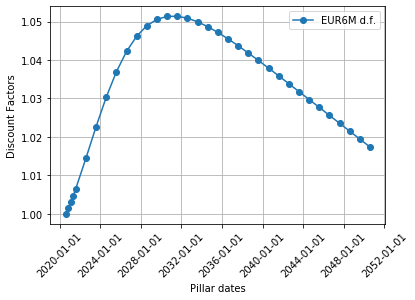
\includegraphics{figures/ex5.5.png}
\end{center}
\end{Answer}




